\documentclass[a4paper,11pt]{article}
\usepackage{f420}

\captionsetup{width=0.8\textwidth}

\begin{document}

\section{\bf Range-деревья}

\emph{Range-дерево (дерево параллелепипедов)}~— структура данных, позволяющая
хранить \(n\)~то\-чек \(p_1, p_2, \ldots, p_n \in \br^d\) и отвечать на
запросы вида «сколько точек \(p_i\) находится в параллелепипеде
\([x^1_1, x^1_2] \times \ldots \times [x^d_1, x^d_2]\)»
за время \(O (\log^{d-1} n)\); при этом построение структуры данных
для \(n\) точек занимает время \(O (n \cdot \log^{d-1} n)\).

При \(d \ge 2\) \(d\)-мерное дерево параллелепипедов устроено следующим
образом: это дерево отрезков для множества всех точек, упорядоченного по
первой координате, в каждой вершине которого хранится,
для множества всех точек \(p_i\) в листьях–потомках данной вершины,
\begin{itemize}
  \item их количество;
  \item наибольшее и наименьшее значение их первой координаты;
  \item \(d-1\)-мерное дерево параллелепипедов по оставшимся \(d-1\)
    координатам, кроме первой.
\end{itemize}

Дерево параллелепипедов размерности \(d-1\), построенное в данной
вершине \(d\)-мерного дерева для множества точек в её поддереве,
называется \emph{ассоциированной структурой},
см.~рисунок~\ref{fig:range-tree}.

\begin{figure}[h] \centering
  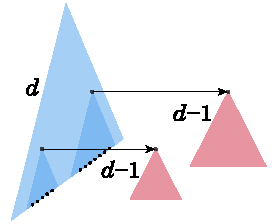
\includegraphics{img/range-tree}
  \caption{Ассоциированные структуры: в каждом внутреннем узле
    \(d\)-мерного дерева параллелепипедов~— \(d-1\)-мерное
    дерево, построенное для множества всех точек \(p_i\) под данным узлом}
  \label{fig:range-tree}
\end{figure}

Так как \(d\)-мерное дерево по сути \emph{состоит} из \(d-1\)-мерных,
то понимать, какое время требуется на построение и на запрос,
мы будем индукцией по размерности. Только \emph{базой индукции}
будет случай \(d = 2\): для двумерного дерева мы покажем, как его
можно нетривиально ускорить.

\begin{theorem}
  Пусть \(d \ge 3\); запрос к \(d\)-мерному дереву параллелепипедов
  сводится к \(\log n\) запросам к \(d-1\)-мерным деревьям.
\end{theorem}

\begin{proof}
Сначала вспомним, как устроен запрос к одномерному дереву
отрезков~— а устроен он следующим образом. Будем рекурсивно
спускаться из корня, и в текущей вершине для каждого из двух детей:
\begin{itemize}
  \item если отрезок, накрываемый им, не пересекает диапазон
    из запроса, — не вызываемся от этого ребёнка,
  \item если отрезок, накрываемый им, полностью содержится в диапазоне
    из запроса, — прибавляем к ответу количество точек, находящихся
    в листьях под этим ребёнком (это количество хранится
    непосредственно в нём);
  \item если отрезок, накрываемый им, пересекается с диапазоном
    из запроса, — вызываемся от него рекурсивно.
\end{itemize}

В общем, дерево отрезков в точности накрывает диапазон из запроса
поддеревьями \(\log n\) своих узлов, и ответ на запрос~— сумма
хранящихся в этих узлах количеств точек в листьях их поддерева.

Пусть теперь мы отвечаем на \(d\)-мерный запрос
\([x^1_1, x^1_2] \times \ldots \times [x^d_1, x^d_2]\).
Наше дерево параллелепипедов~— оно же дерево отрезков по первой
координате. Потому мы можем, как описано выше, накрыть множество
точек \(p_i\), первая координата которых лежит в отрезке
\([x^1_1, x^1_2]\), \(\log n\) вершинами дерева.

После этого останется из множеств точек \(p_i\) под каждой
из этих вершин отфильтровать те, оставшиеся координаты которых
лежат в интересующих нас диапазонах. Это можно сделать
как раз запросами к \(d-1\)-мерным деревьям.
\end{proof}

\begin{theorem}
  Пусть \(d \ge 3\). Если \(d-1\)-мерное дерево отрезков
  для \(n\) точек строится за время \(O (n \cdot \log^{d-2} n)\),
  то \(d\)-мерное дерево отрезков для \(n\) точек строится
  за время \(O (n \cdot \log^{d-1} n)\).
\end{theorem}

\begin{proof}  \begin{multline*}
  T(n)\ =\ 2 \cdot T \lr*{\frac n 2} + O (n \cdot \log^{d-2} n)\ =\ 
  \sum_{k = 0}^{\log n} 2^k \cdot \frac{n}{2^k} \cdot
    \log^{d-2} \lr*{\frac{n}{2^k}}\ = \\
  =\ n \cdot \lr*{\log^{d-2} n + \lr*{\log^{d-2} n}
    + \ldots + 1^{d-2}}
  \ =\ n \cdot \log^{d-1} n.
\end{multline*}  \end{proof}

\begin{theorem}
  Двумерное дерево параллелепипедов можно построить за время
  \(O (n \cdot \log n)\), а отвечать на запросы к нему~—
  за время \(O (\log n)\).
\end{theorem}

\begin{proof}
  То, что описано далее, гуглить/искать в [de Berg, van Kreveld et al.]
  по ключевым словам \emph{``fractional cascading''}.
  Для быстрого построения сначала упорядочим все точки по
  \emph{второй} координате, и в каждой вершине будем хранить \emph{массив}
  из всех точек (вместо одномерного дерева отрезков на них).

  Заметим, что массивы в потомках любой вершины являются подмножествами
  массива в ней. Потому, чтобы быстро отвечать на запрос,
  мы сначала найдём границы диапазона из запроса
  (по второй координате) в массиве в корне (двоичным поиском
  за \(O (\log n)\)). А затем будем получать границы этого диапазона
  в массиве в каждой из вершин, посещённых нами при запросе к дереву
  отрезков, без необходимости осуществлять там поиск.

  Чтобы иметь возможность так сделать, строим дерево следующим образом
  (см.~рисунок~\ref{fig:range-tikz}): упорядоченный по второй координате массив
  в каждой из вершин будем разбивать на две половины по первой координате,
  найдя по ней медиану, за линейное время. После чего каждый элемент\
  соединим ссылкой с \emph{первым элементом с не меньшей второй координатой}
  в каждом из массивов в детях, также за линию. Время на построение~—
  \(T(n) = 2T(\frac n 2) + O(n) = O(n \cdot \log n)\).

  При ответе на запрос будем переходить по ссылкам из крайних элементов
  диапазона по второй координате в вершины, которые посещает запрос
  к дереву отрезков по первой координате. Если ссылка из правого края
  пришла в элемент, не входящий в диапазон запроса по второй координате,
  отступим в массиве на один элемент влево. Время на запрос~— \(O (\log n)\)
  на двоичный поиск в массиве в корне и \(O (\log n)\) переходов по ссылкам.
\end{proof}

\begin{figure} \centering
  \newcommand{\vs}[2]{\(\begin{matrix} #1 \\ #2 \end{matrix}\)}
\newcommand{\nvs}[2]{node[right,rectangle,fill=white,fill opacity=0.8,inner sep=0.2mm]{\vs{#1}{#2}}}
\newcommand{\ns}{node[circle,fill=white,inner sep=0.1mm]{\tiny \(\varnothing\)}}

\begin{tikzpicture}[scale=0.5,rotate=-90]
  \fill[PaleGreen,opacity=0.5] (4.5,2.5) rectangle (12.5,11.5);
  \draw[very thick] (-0.5,-0.5) rectangle ++(16,16) (7.5,-0.5) -- ++(0,16);
  \draw[very thick, dashed] (3.5,-0.5) -- ++(0,16) (11.5,-0.5) -- ++(0,16);
  \draw \foreach \x in {2,6,10,14} {(\x-0.5,-0.5) -- ++(0,16)};
  \draw[dashed] \foreach \x in {1,3,5,7,9,11,13,15} {(\x-0.5,-0.5) -- ++(0,16)};

  \draw (2, 0) \nvs{2}{0} node[circle,fill=black,inner sep=0.4mm]{};
  \draw (10, 1) \nvs{10}{1} node[circle,fill=black,inner sep=0.4mm]{};
  \draw (0, 2) \nvs{0}{2} node[circle,fill=black,inner sep=0.4mm]{};
  \draw (11, 3) \nvs{11}{3} node[circle,fill=black,inner sep=0.4mm]{};
  \draw (13, 4) \nvs{13}{4} node[circle,fill=black,inner sep=0.4mm]{};
  \draw (3, 5) \nvs{3}{5} node[circle,fill=black,inner sep=0.4mm]{};
  \draw (7, 6) \nvs{7}{6} node[circle,fill=black,inner sep=0.4mm]{};
  \draw (12, 7) \nvs{12}{7} node[circle,fill=black,inner sep=0.4mm]{};
  \draw (15, 8) \nvs{15}{8} node[circle,fill=black,inner sep=0.4mm]{};
  \draw (5, 9) \nvs{5}{9} node[circle,fill=black,inner sep=0.4mm]{};
  \draw (6, 10) \nvs{6}{10} node[circle,fill=black,inner sep=0.4mm]{};
  \draw (9, 11) \nvs{9}{11} node[circle,fill=black,inner sep=0.4mm]{};
  \draw (8, 12) \nvs{8}{12} node[circle,fill=black,inner sep=0.4mm]{};
  \draw (4, 13) \nvs{4}{13} node[circle,fill=black,inner sep=0.4mm]{};
  \draw (14, 14) \nvs{14}{14} node[circle,fill=black,inner sep=0.4mm]{};
  \draw (1, 15) \nvs{1}{15} node[circle,fill=black,inner sep=0.4mm]{};
\end{tikzpicture} \vspace{0.4cm}


\begin{tikzpicture}[xscale=0.5]
  \fill[PaleGreen,opacity=0.5] (3,0) rectangle (12,1);
  \draw (0, 0) grid ++(16, 1) (0.5, 0.5)
    node{\vs{2}{0}} ++(1,0)
    node{\vs{10}{1}} ++(1,0)
    node{\vs{0}{2}} ++(1,0)
    node{\vs{11}{3}} ++(1,0)
    node{\vs{13}{4}} ++(1,0)
    node{\vs{3}{5}} ++(1,0)
    node{\vs{7}{6}} ++(1,0)
    node{\vs{12}{7}} ++(1,0)
    node{\vs{15}{8}} ++(1,0)
    node{\vs{5}{9}} ++(1,0)
    node{\vs{6}{10}} ++(1,0)
    node{\vs{9}{11}} ++(1,0)
    node{\vs{8}{12}} ++(1,0)
    node{\vs{4}{13}} ++(1,0)
    node{\vs{14}{14}} ++(1,0)
    node{\vs{1}{15}} ++(1,0);
  \draw[very thick] (0.3, 0) .. controls (0.3, -1) and (-3.5, -1) .. (-3.5, -2);
  \draw (0.7, 0) .. controls (0.7, -1) and (12.5, -1) .. (12.5, -2);
  \draw[very thick] (1.3, 0) .. controls (1.3, -1) and (-2.5, -1) .. (-2.5, -2);
  \draw (1.7, 0) .. controls (1.7, -1) and (12.5, -1) .. (12.5, -2);
  \draw[very thick] (2.3, 0) .. controls (2.3, -1) and (-2.5, -1) .. (-2.5, -2);
  \draw (2.7, 0) .. controls (2.7, -1) and (13.5, -1) .. (13.5, -2);
  \draw[very thick,LimeGreen] (3.3, 0) .. controls (3.3, -1) and (-1.5, -1) .. (-1.5, -2);
  \draw[very thick,LimeGreen] (3.7, 0) .. controls (3.7, -1) and (13.5, -1) .. (13.5, -2);
  \draw[very thick,LimeGreen] (4.3, 0) .. controls (4.3, -1) and (-1.5, -1) .. (-1.5, -2);
  \draw[very thick,LimeGreen] (4.7, 0) .. controls (4.7, -1) and (14.5, -1) .. (14.5, -2);
  \draw[very thick,LimeGreen] (5.3, 0) .. controls (5.3, -1) and (-1.5, -1) .. (-1.5, -2);
  \draw[very thick,LimeGreen] (5.7, 0) .. controls (5.7, -1) and (15.5, -1) .. (15.5, -2);
  \draw[very thick,LimeGreen] (6.3, 0) .. controls (6.3, -1) and (-0.5, -1) .. (-0.5, -2);
  \draw[very thick,LimeGreen] (6.7, 0) .. controls (6.7, -1) and (15.5, -1) .. (15.5, -2);
  \draw[very thick,LimeGreen] (7.3, 0) .. controls (7.3, -1) and (0.5, -1) .. (0.5, -2);
  \draw[very thick,LimeGreen] (7.7, 0) .. controls (7.7, -1) and (15.5, -1) .. (15.5, -2);
  \draw[very thick,LimeGreen] (8.3, 0) .. controls (8.3, -1) and (0.5, -1) .. (0.5, -2);
  \draw[very thick,LimeGreen] (8.7, 0) .. controls (8.7, -1) and (16.5, -1) .. (16.5, -2);
  \draw[very thick,LimeGreen] (9.3, 0) .. controls (9.3, -1) and (0.5, -1) .. (0.5, -2);
  \draw[very thick,LimeGreen] (9.7, 0) .. controls (9.7, -1) and (17.5, -1) .. (17.5, -2);
  \draw[very thick,LimeGreen] (10.3, 0) .. controls (10.3, -1) and (1.5, -1) .. (1.5, -2);
  \draw[very thick,LimeGreen] (10.7, 0) .. controls (10.7, -1) and (17.5, -1) .. (17.5, -2);
  \draw[very thick,LimeGreen,->]
    (11.3, 0) .. controls (11.3, -1) and (2.5, -1) .. (2.5, -2) -- ++(-1,0);
  \draw[very thick,LimeGreen] (11.7, 0) .. controls (11.7, -1) and (17.5, -1) .. (17.5, -2);
  \draw[very thick] (12.3, 0) .. controls (12.3, -1) and (2.5, -1) .. (2.5, -2);
  \draw (12.7, 0) .. controls (12.7, -1) and (18.5, -1) .. (18.5, -2);
  \draw[very thick] (13.3, 0) .. controls (13.3, -1) and (2.5, -1) .. (2.5, -2);
  \draw (13.7, 0) .. controls (13.7, -1) and (19.5, -1) .. (19.5, -2);
  \draw[very thick] (14.3, 0) .. controls (14.3, -1) and (3.5, -1) .. (3.5, -2);
  \draw (14.7, 0) .. controls (14.7, -1) and (19.5, -1) .. (19.5, -2);
  \draw[very thick] (15.3, 0) .. controls (15.3, -1) and (3.5, -1) .. (3.5, -2);
  \draw (15.7, 0) -- ++(0, -0.5) \ns;
  \fill[PaleGreen,opacity=0.5] (-2,-3) rectangle (2,-2);
  \draw (-4, -3) grid ++(8, 1) (-3.5, -2.5)
    node{\vs{2}{0}} ++(1,0)
    node{\vs{0}{2}} ++(1,0)
    node{\vs{3}{5}} ++(1,0)
    node{\vs{7}{6}} ++(1,0)
    node{\vs{5}{9}} ++(1,0)
    node{\vs{6}{10}} ++(1,0)
    node{\vs{4}{13}} ++(1,0)
    node{\vs{1}{15}} ++(1,0);
  \draw[very thick] (-3.7, -3) .. controls (-3.7, -4) and (-5.5, -4) .. (-5.5, -5);
  \draw (-3.3, -3) .. controls (-3.3, -4) and (2.5, -4) .. (2.5, -5);
  \draw[very thick] (-2.7, -3) .. controls (-2.7, -4) and (-4.5, -4) .. (-4.5, -5);
  \draw (-2.3, -3) .. controls (-2.3, -4) and (2.5, -4) .. (2.5, -5);
  \draw[very thick] (-1.7, -3) .. controls (-1.7, -4) and (-3.5, -4) .. (-3.5, -5);
  \draw[very thick,LimeGreen] (-1.3, -3) .. controls (-1.3, -4) and (2.5, -4) .. (2.5, -5);
  \draw[very thick] (-0.7, -3) .. controls (-0.7, -4) and (-2.5, -4) .. (-2.5, -5);
  \draw[very thick,LimeGreen] (-0.3, -3) .. controls (-0.3, -4) and (2.5, -4) .. (2.5, -5);
  \draw[very thick] (0.3, -3) .. controls (0.3, -4) and (-2.5, -4) .. (-2.5, -5);
  \draw[very thick,LimeGreen] (0.7, -3) .. controls (0.7, -4) and (3.5, -4) .. (3.5, -5);
  \draw[very thick] (1.3, -3) .. controls (1.3, -4) and (-2.5, -4) .. (-2.5, -5);
  \draw[very thick,LimeGreen] (1.7, -3) .. controls (1.7, -4) and (4.5, -4) .. (4.5, -5);
  \draw[very thick] (2.3, -3) .. controls (2.3, -4) and (-2.5, -4) .. (-2.5, -5);
  \draw (2.7, -3) .. controls (2.7, -4) and (5.5, -4) .. (5.5, -5);
  \draw[very thick] (3.3, -3) .. controls (3.3, -4) and (-2.5, -4) .. (-2.5, -5);
  \draw (3.7, -3) -- ++(0, -0.5) \ns;
  \draw (-6, -6) grid ++(4, 1) (-5.5, -5.5)
    node{\vs{2}{0}} ++(1,0)
    node{\vs{0}{2}} ++(1,0)
    node{\vs{3}{5}} ++(1,0)
    node{\vs{1}{15}} ++(1,0);
  \draw[very thick] (-5.7, -6) .. controls (-5.7, -7) and (-6.5, -7) .. (-6.5, -8);
  \draw (-5.3, -6) .. controls (-5.3, -7) and (-2.5, -7) .. (-2.5, -8);
  \draw[very thick] (-4.7, -6) .. controls (-4.7, -7) and (-6.5, -7) .. (-6.5, -8);
  \draw (-4.3, -6) .. controls (-4.3, -7) and (-1.5, -7) .. (-1.5, -8);
  \draw[very thick] (-3.7, -6) .. controls (-3.7, -7) and (-5.5, -7) .. (-5.5, -8);
  \draw (-3.3, -6) .. controls (-3.3, -7) and (-1.5, -7) .. (-1.5, -8);
  \draw[very thick] (-2.7, -6) .. controls (-2.7, -7) and (-5.5, -7) .. (-5.5, -8);
  \draw (-2.3, -6) -- ++(0, -0.5) \ns;
  \draw (-7, -9) grid ++(2, 1) (-6.5, -8.5)
    node{\vs{0}{2}} ++(1,0)
    node{\vs{1}{15}} ++(1,0);
  \draw[very thick] (-6.7, -9) .. controls (-6.7, -10) and (-7, -10) .. (-7, -11);
  \draw (-6.3, -9) .. controls (-6.3, -10) and (-5, -10) .. (-5, -11);
  \draw[very thick] (-5.7, -9) -- ++(0, -0.5) \ns;
  \draw (-5.3, -9) .. controls (-5.3, -10) and (-5, -10) .. (-5, -11);
  \draw (-7.5, -12) rectangle ++(1, 1) (-7, -11.5)
    node{\vs{0}{2}} ++(1,0);
  \draw (-5.5, -12) rectangle ++(1, 1) (-5, -11.5)
    node{\vs{1}{15}} ++(1,0);
  \draw (-3, -9) grid ++(2, 1) (-2.5, -8.5)
    node{\vs{2}{0}} ++(1,0)
    node{\vs{3}{5}} ++(1,0);
  \draw[very thick] (-2.7, -9) .. controls (-2.7, -10) and (-3, -10) .. (-3, -11);
  \draw (-2.3, -9) .. controls (-2.3, -10) and (-1, -10) .. (-1, -11);
  \draw[very thick] (-1.7, -9) -- ++(0, -0.5) \ns;
  \draw (-1.3, -9) .. controls (-1.3, -10) and (-1, -10) .. (-1, -11);
  \draw (-3.5, -12) rectangle ++(1, 1) (-3, -11.5)
    node{\vs{2}{0}} ++(1,0);
  \draw (-1.5, -12) rectangle ++(1, 1) (-1, -11.5)
    node{\vs{3}{5}} ++(1,0);
  \fill[PaleGreen,opacity=0.5] (2,-6) rectangle (5,-5);
  \draw (2, -6) grid ++(4, 1) (2.5, -5.5)
    node{\vs{7}{6}} ++(1,0)
    node{\vs{5}{9}} ++(1,0)
    node{\vs{6}{10}} ++(1,0)
    node{\vs{4}{13}} ++(1,0);
  \draw[very thick,LimeGreen] (2.3, -6) .. controls (2.3, -7) and (1.5, -7) .. (1.5, -8);
  \draw[very thick,LimeGreen] (2.7, -6) .. controls (2.7, -7) and (5.5, -7) .. (5.5, -8);
  \draw[very thick,LimeGreen] (3.3, -6) .. controls (3.3, -7) and (1.5, -7) .. (1.5, -8);
  \draw[very thick,LimeGreen] (3.7, -6) .. controls (3.7, -7) and (6.5, -7) .. (6.5, -8);
  \draw[very thick,LimeGreen,->]
    (4.3, -6) .. controls (4.3, -7) and (2.5, -7) .. (2.5, -8) -- ++(-1,0);
  \draw[very thick,LimeGreen] (4.7, -6) .. controls (4.7, -7) and (6.5, -7) .. (6.5, -8);
  \draw[very thick] (5.3, -6) .. controls (5.3, -7) and (2.5, -7) .. (2.5, -8);
  \draw (5.7, -6) -- ++(0, -0.5) \ns;
  \fill[PaleGreen,opacity=0.5] (1,-9) rectangle (2,-8);
  \draw (1, -9) grid ++(2, 1) (1.5, -8.5)
    node{\vs{5}{9}} ++(1,0)
    node{\vs{4}{13}} ++(1,0);
  \draw[very thick] (1.3, -9) .. controls (1.3, -10) and (1, -10) .. (1, -11);
  \draw[very thick,LimeGreen] (1.7, -9) .. controls (1.7, -10) and (3, -10) .. (3, -11);
  \draw[very thick] (2.3, -9) .. controls (2.3, -10) and (1, -10) .. (1, -11);
  \draw (2.7, -9) -- ++(0, -0.5) \ns;
  \draw (0.5, -12) rectangle ++(1, 1) (1, -11.5)
    node{\vs{4}{13}} ++(1,0);
  \filldraw[fill=PaleGreen,fill opacity=0.5,very thick,draw=MediumBlue]
    (2.5, -12) rectangle ++(1, 1);
  \draw (3, -11.5) node{\vs{5}{9}};
  \fill[PaleGreen,opacity=0.5] (5,-9) rectangle (7,-8);
  \draw[very thick,MediumBlue] (5, -9) grid ++(2, 1); \draw (5.5, -8.5)
    node{\vs{7}{6}} ++(1,0)
    node{\vs{6}{10}};
  \draw[very thick] (5.3, -9) .. controls (5.3, -10) and (5, -10) .. (5, -11);
  \draw[very thick,LimeGreen] (5.7, -9) .. controls (5.7, -10) and (7, -10) .. (7, -11);
  \draw[very thick] (6.3, -9) .. controls (6.3, -10) and (5, -10) .. (5, -11);
  \draw[very thick,LimeGreen] (6.7, -9) -- ++(0, -0.5) \ns;
  \draw (4.5, -12) rectangle ++(1, 1) (5, -11.5)
    node{\vs{6}{10}} ++(1,0);
  \draw (6.5, -12) rectangle ++(1, 1) (7, -11.5)
    node{\vs{7}{6}} ++(1,0);
  \fill[PaleGreen,opacity=0.5] (13,-3) rectangle (18,-2);
  \draw (12, -3) grid ++(8, 1) (12.5, -2.5)
    node{\vs{10}{1}} ++(1,0)
    node{\vs{11}{3}} ++(1,0)
    node{\vs{13}{4}} ++(1,0)
    node{\vs{12}{7}} ++(1,0)
    node{\vs{15}{8}} ++(1,0)
    node{\vs{9}{11}} ++(1,0)
    node{\vs{8}{12}} ++(1,0)
    node{\vs{14}{14}} ++(1,0);
  \draw[very thick] (12.3, -3) .. controls (12.3, -4) and (10.5, -4) .. (10.5, -5);
  \draw (12.7, -3) .. controls (12.7, -4) and (18.5, -4) .. (18.5, -5);
  \draw[very thick,LimeGreen] (13.3, -3) .. controls (13.3, -4) and (11.5, -4) .. (11.5, -5);
  \draw[very thick,LimeGreen] (13.7, -3) .. controls (13.7, -4) and (18.5, -4) .. (18.5, -5);
  \draw[very thick,LimeGreen] (14.3, -3) .. controls (14.3, -4) and (12.5, -4) .. (12.5, -5);
  \draw[very thick,LimeGreen] (14.7, -3) .. controls (14.7, -4) and (18.5, -4) .. (18.5, -5);
  \draw[very thick,LimeGreen] (15.3, -3) .. controls (15.3, -4) and (12.5, -4) .. (12.5, -5);
  \draw[very thick,LimeGreen] (15.7, -3) .. controls (15.7, -4) and (19.5, -4) .. (19.5, -5);
  \draw[very thick,LimeGreen] (16.3, -3) .. controls (16.3, -4) and (12.5, -4) .. (12.5, -5);
  \draw[very thick,LimeGreen] (16.7, -3) .. controls (16.7, -4) and (20.5, -4) .. (20.5, -5);
  \draw[very thick,LimeGreen] (17.3, -3) .. controls (17.3, -4) and (12.5, -4) .. (12.5, -5);
  \draw[very thick,LimeGreen,->]
    (17.7, -3) .. controls (17.7, -4) and (21.5, -4) .. (21.5, -5) -- ++(-1,0);
  \draw[very thick] (18.3, -3) .. controls (18.3, -4) and (13.5, -4) .. (13.5, -5);
  \draw (18.7, -3) .. controls (18.7, -4) and (21.5, -4) .. (21.5, -5);
  \draw[very thick] (19.3, -3) -- ++(0, -0.5) \ns;
  \draw (19.7, -3) .. controls (19.7, -4) and (21.5, -4) .. (21.5, -5);
  \fill[PaleGreen,opacity=0.5] (11,-6) rectangle (13,-5);
  \draw[very thick,MediumBlue] (10, -6) grid ++(4, 1); \draw (10.5, -5.5)
    node{\vs{10}{1}} ++(1,0)
    node{\vs{11}{3}} ++(1,0)
    node{\vs{9}{11}} ++(1,0)
    node{\vs{8}{12}};
  \draw[very thick] (10.3, -6) .. controls (10.3, -7) and (9.5, -7) .. (9.5, -8);
  \draw (10.7, -6) .. controls (10.7, -7) and (13.5, -7) .. (13.5, -8);
  \draw[very thick] (11.3, -6) .. controls (11.3, -7) and (9.5, -7) .. (9.5, -8);
  \draw (11.7, -6) .. controls (11.7, -7) and (14.5, -7) .. (14.5, -8);
  \draw[very thick] (12.3, -6) .. controls (12.3, -7) and (9.5, -7) .. (9.5, -8);
  \draw (12.7, -6) -- ++(0, -0.5) \ns;
  \draw[very thick] (13.3, -6) .. controls (13.3, -7) and (10.5, -7) .. (10.5, -8);
  \draw (13.7, -6) -- ++(0, -0.5) \ns;
  \draw (9, -9) grid ++(2, 1) (9.5, -8.5)
    node{\vs{9}{11}} ++(1,0)
    node{\vs{8}{12}} ++(1,0);
  \draw[very thick] (9.3, -9) .. controls (9.3, -10) and (9, -10) .. (9, -11);
  \draw (9.7, -9) .. controls (9.7, -10) and (11, -10) .. (11, -11);
  \draw[very thick] (10.3, -9) .. controls (10.3, -10) and (9, -10) .. (9, -11);
  \draw (10.7, -9) -- ++(0, -0.5) \ns;
  \draw (8.5, -12) rectangle ++(1, 1) (9, -11.5)
    node{\vs{8}{12}} ++(1,0);
  \draw (10.5, -12) rectangle ++(1, 1) (11, -11.5)
    node{\vs{9}{11}} ++(1,0);
  \draw (13, -9) grid ++(2, 1) (13.5, -8.5)
    node{\vs{10}{1}} ++(1,0)
    node{\vs{11}{3}} ++(1,0);
  \draw[very thick] (13.3, -9) .. controls (13.3, -10) and (13, -10) .. (13, -11);
  \draw (13.7, -9) .. controls (13.7, -10) and (15, -10) .. (15, -11);
  \draw[very thick] (14.3, -9) -- ++(0, -0.5) \ns;
  \draw (14.7, -9) .. controls (14.7, -10) and (15, -10) .. (15, -11);
  \draw (12.5, -12) rectangle ++(1, 1) (13, -11.5)
    node{\vs{10}{1}} ++(1,0);
  \draw (14.5, -12) rectangle ++(1, 1) (15, -11.5)
    node{\vs{11}{3}} ++(1,0);
  \fill[PaleGreen,opacity=0.5] (18,-6) rectangle (21,-5);
  \draw (18, -6) grid ++(4, 1) (18.5, -5.5)
    node{\vs{13}{4}} ++(1,0)
    node{\vs{12}{7}} ++(1,0)
    node{\vs{15}{8}} ++(1,0)
    node{\vs{14}{14}} ++(1,0);
  \draw[very thick,LimeGreen] (18.3, -6) .. controls (18.3, -7) and (17.5, -7) .. (17.5, -8);
  \draw (18.7, -6) .. controls (18.7, -7) and (21.5, -7) .. (21.5, -8);
  \draw[very thick,LimeGreen] (19.3, -6) .. controls (19.3, -7) and (18.5, -7) .. (18.5, -8);
  \draw (19.7, -6) .. controls (19.7, -7) and (21.5, -7) .. (21.5, -8);
  \draw[very thick] (20.3, -6) -- ++(0, -0.5) \ns;
  \draw (20.7, -6) .. controls (20.7, -7) and (21.5, -7) .. (21.5, -8);
  \draw[very thick] (21.3, -6) -- ++(0, -0.5) \ns;
  \draw (21.7, -6) .. controls (21.7, -7) and (22.5, -7) .. (22.5, -8);
  \fill[PaleGreen,opacity=0.5] (17,-9) rectangle (19,-8);
  \draw (17, -9) grid ++(2, 1) (17.5, -8.5)
    node{\vs{13}{4}} ++(1,0)
    node{\vs{12}{7}} ++(1,0);
  \draw[very thick,LimeGreen] (17.3, -9) .. controls (17.3, -10) and (17, -10) .. (17, -11);
  \draw (17.7, -9) .. controls (17.7, -10) and (19, -10) .. (19, -11);
  \draw[very thick,LimeGreen] (18.3, -9) .. controls (18.3, -10) and (17, -10) .. (17, -11);
  \draw (18.7, -9) -- ++(0, -0.5) \ns;
  \filldraw[fill=PaleGreen,fill opacity=0.5,very thick,draw=MediumBlue]
    (16.5, -12) rectangle ++(1, 1);
  \draw (17, -11.5) node{\vs{12}{7}};
  \draw (18.5, -12) rectangle ++(1, 1) (19, -11.5)
    node{\vs{13}{4}} ++(1,0);
  \draw (21, -9) grid ++(2, 1) (21.5, -8.5)
    node{\vs{15}{8}} ++(1,0)
    node{\vs{14}{14}} ++(1,0);
  \draw[very thick] (21.3, -9) .. controls (21.3, -10) and (21, -10) .. (21, -11);
  \draw (21.7, -9) .. controls (21.7, -10) and (23, -10) .. (23, -11);
  \draw[very thick] (22.3, -9) .. controls (22.3, -10) and (21, -10) .. (21, -11);
  \draw (22.7, -9) -- ++(0, -0.5) \ns;
  \draw (20.5, -12) rectangle ++(1, 1) (21, -11.5)
    node{\vs{14}{14}} ++(1,0);
  \draw (22.5, -12) rectangle ++(1, 1) (23, -11.5)
    node{\vs{15}{8}} ++(1,0);
\end{tikzpicture}


  \caption{Множество точек в \(\br^2\), границы дерева отрезков по первой координате
    и запрос \([5, 12] \times [3, 9]\) (вверху, координаты «матричные»);
    двумерное дерево параллелепипедов и переходы по ссылкам, соответствующие
    обработке этого запроса (внизу)}
  \label{fig:range-tikz}
\end{figure}

\end{document}
